\documentclass[10pt]{article}
\usepackage[paperwidth=960pt, paperheight=540pt, margin=16pt]{geometry}
\usepackage[utf8]{inputenc}
\usepackage[T1]{fontenc}
\usepackage{lmodern}
\usepackage{amsmath,amssymb}
\usepackage{graphicx}
\usepackage{xcolor}
\usepackage{tcolorbox}
\tcbuselibrary{skins}

\definecolor{darkblue}{RGB}{10, 37, 64}
\definecolor{primaryblue}{RGB}{24, 76, 120}
\definecolor{lightbg}{RGB}{248, 250, 252}
\definecolor{borderblue}{RGB}{203, 213, 225}
\definecolor{accentgreen}{RGB}{16, 120, 72}

\pagestyle{empty}

\begin{document}

% ==================== Slide 1 ====================
\begin{center}
  \fboxsep=0pt\fboxrule=0.7pt\relax
  \fcolorbox{borderblue}{white}{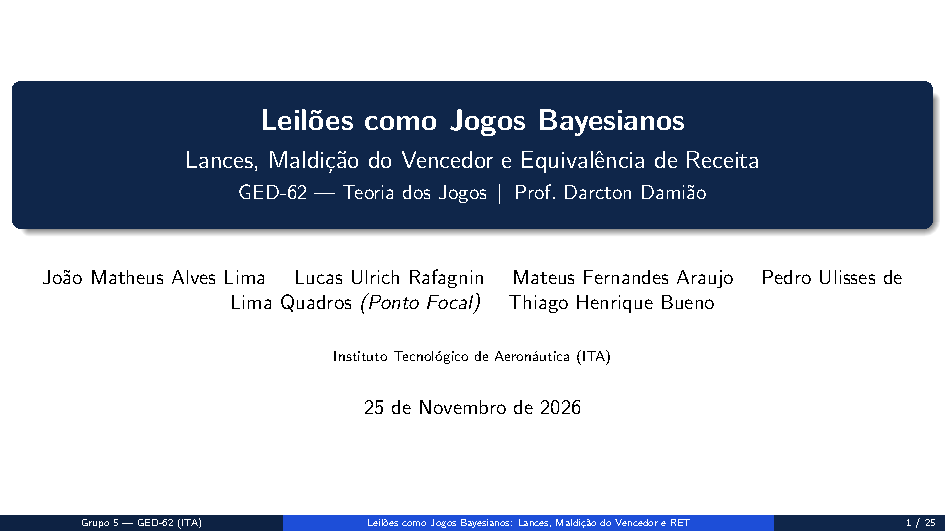
\includegraphics[page=1, width=0.48\textwidth]{main.pdf}}
\end{center}
\vspace{4pt}
\begin{tcolorbox}[
    enhanced,
    colback=lightbg,
    colframe=primaryblue,
    arc=3pt,
    boxrule=0.8pt,
    left=12pt, right=12pt, top=7pt, bottom=7pt
]
  \textbf{\color{accentgreen}[TEMPO: 00:00 -- 00:40 \textbar\ 40 s]} \hfill
  \textbf{\color{gray}Slide 1 de 25 \textbar\ Capa do Trabalho}
  \vspace{3pt}\hrule\vspace{5pt}
  {\linespread{1.06}\footnotesize
  ``Bom dia, professor Darcton, bom dia colegas de turma. Somos o Grupo 5 de Teoria dos Jogos (GED-62), e hoje apresentamos nosso trabalho final sobre \textbf{Leil\~oes como Jogos Bayesianos: Lances, Maldi\c{c}\~ao do Vencedor e Equival\^encia de Receita}. O objetivo desta apresenta\c{c}\~ao \'e mostrar como a Teoria dos Jogos modela rigorosamente situa\c{c}\~oes em que os agentes tomam decis\~oes estrat\'egicas sob informa\c{c}\~ao incompleta, culminando na aplica\c{c}\~ao pr\'atica aos leil\~oes bilion\'arios de publicidade digital da internet.''
  }
\end{tcolorbox}
\newpage

% ==================== Slide 2 ====================
\begin{center}
  \fboxsep=0pt\fboxrule=0.7pt\relax
  \fcolorbox{borderblue}{white}{\includegraphics[page=2, width=0.48\textwidth]{main.pdf}}
\end{center}
\vspace{4pt}
\begin{tcolorbox}[
    enhanced,
    colback=lightbg,
    colframe=primaryblue,
    arc=3pt,
    boxrule=0.8pt,
    left=12pt, right=12pt, top=7pt, bottom=7pt
]
  \textbf{\color{accentgreen}[TEMPO: 00:40 -- 01:15 \textbar\ 35 s]} \hfill
  \textbf{\color{gray}Slide 2 de 25 \textbar\ Roteiro da Apresenta\c{c}\~ao}
  \vspace{3pt}\hrule\vspace{5pt}
  {\linespread{1.06}\footnotesize
  ``Para cumprir o tempo de 30 minutos com clareza e rigor metodol\'ogico, estruturamos nossa exposi\c{c}\~ao em quatro etapas fundamentais: primeiro, a \textbf{Fundamenta\c{c}\~ao Te\'orica}, onde construiremos os conceitos de tipo privado, ENB, os quatro formatos cl\'assicos e o Teorema da Equival\^encia de Receita; segundo, o \textbf{Modelo Resolvido Passo a Passo}, onde demonstraremos a resolu\c{c}\~ao anal\'itica da EDO de equil\'ibrio e a compara\c{c}\~ao de receitas; terceiro, o \textbf{Caso Real}, analisando as transi\c{c}\~oes de mercado da publicidade online em 2002 e 2019; e, finalmente, a s\'intese de como este tema expande a ementa de GED-62.''
  }
\end{tcolorbox}
\newpage

% ==================== Slide 3 ====================
\begin{center}
  \fboxsep=0pt\fboxrule=0.7pt\relax
  \fcolorbox{borderblue}{white}{\includegraphics[page=3, width=0.48\textwidth]{main.pdf}}
\end{center}
\vspace{4pt}
\begin{tcolorbox}[
    enhanced,
    colback=lightbg,
    colframe=primaryblue,
    arc=3pt,
    boxrule=0.8pt,
    left=12pt, right=12pt, top=7pt, bottom=7pt
]
  \textbf{\color{accentgreen}[TEMPO: 01:15 -- 01:30 \textbar\ 15 s]} \hfill
  \textbf{\color{gray}Slide 3 de 25 \textbar\ Transi\c{c}\~ao: Conceito e Fundamenta\c{c}\~ao Te\'orica}
  \vspace{3pt}\hrule\vspace{5pt}
  {\linespread{1.06}\footnotesize
  ``Entramos agora na Se\c{c}\~ao 1: Conceito e Fundamenta\c{c}\~ao Te\'orica. A seguir, apresentaremos a formaliza\c{c}\~ao matem\'atica que nos permite transitar dos jogos de informa\c{c}\~ao completa para os jogos bayesianos de informa\c{c}\~ao incompleta.''
  }
\end{tcolorbox}
\newpage

% ==================== Slide 4 ====================
\begin{center}
  \fboxsep=0pt\fboxrule=0.7pt\relax
  \fcolorbox{borderblue}{white}{\includegraphics[page=4, width=0.48\textwidth]{main.pdf}}
\end{center}
\vspace{4pt}
\begin{tcolorbox}[
    enhanced,
    colback=lightbg,
    colframe=primaryblue,
    arc=3pt,
    boxrule=0.8pt,
    left=12pt, right=12pt, top=7pt, bottom=7pt
]
  \textbf{\color{accentgreen}[TEMPO: 01:30 -- 02:45 \textbar\ 1 min 15 s]} \hfill
  \textbf{\color{gray}Slide 4 de 25 \textbar\ 1.1. Da Informa\c{c}\~ao Completa ao Jogo Bayesiano}
  \vspace{3pt}\hrule\vspace{5pt}
  {\linespread{1.06}\footnotesize
  ``Na primeira metade de GED-62, estudamos jogos sob a hip\'otese de informa\c{c}\~ao completa, como o Dilema dos Prisioneiros ou o duop\'olio de Cournot com custos marginais p\'ublicos. Nesses modelos, a matriz de payoffs e as fun\c{c}\~oes de utilidade s\~ao de conhecimento comum. Contudo, em transa\c{c}\~oes econ\^omicas reais e em leil\~oes, essa hip\'otese \'e insustent\'avel. Quando uma empresa entra num leil\~ao de frequ\^encias 5G da Anatel ou de concess\~ao de rodovias, ela conhece com exatid\~ao o seu pr\'oprio teto financeiro e sua estrutura de custos, mas os limites dos seus concorrentes s\~ao segredos industriais. Estamos, portanto, em um \textbf{jogo de informa\c{c}\~ao incompleta}. A grande quest\~ao conceitual \'e: como modelar o equil\'ibrio quando voc\^e nem sequer tem certeza de qual fun\c{c}\~ao de payoff o seu advers\'ario est\'a maximizando?''
  }
\end{tcolorbox}
\newpage

% ==================== Slide 5 ====================
\begin{center}
  \fboxsep=0pt\fboxrule=0.7pt\relax
  \fcolorbox{borderblue}{white}{\includegraphics[page=5, width=0.48\textwidth]{main.pdf}}
\end{center}
\vspace{4pt}
\begin{tcolorbox}[
    enhanced,
    colback=lightbg,
    colframe=primaryblue,
    arc=3pt,
    boxrule=0.8pt,
    left=12pt, right=12pt, top=7pt, bottom=7pt
]
  \textbf{\color{accentgreen}[TEMPO: 02:45 -- 04:05 \textbar\ 1 min 20 s]} \hfill
  \textbf{\color{gray}Slide 5 de 25 \textbar\ 1.2. A Transforma\c{c}\~ao de Harsanyi: Tipo Privado e Prior Comum}
  \vspace{3pt}\hrule\vspace{5pt}
  {\linespread{1.06}\footnotesize
  ``A resposta a esse dilema foi formulada por John Harsanyi em 1967, rendendo-lhe o Pr\^emio Nobel em 1994. Harsanyi percebeu que poder\'iamos converter esse jogo de informa\c{c}\~ao incompleta em um jogo de informa\c{c}\~ao imperfeita introduzindo um jogador fict\'icio: a \textbf{Natureza}. A Natureza joga primeiro, no `est\'agio zero', sorteando para cada jogador um vetor de caracter\'isticas secretas, denominado \textbf{tipo} $\theta_i$. No nosso caso de leil\~oes, o tipo nada mais \'e do que a valora\c{c}\~ao privada $v_i$ do participante. O segundo pilar indispens\'avel \'e a \textbf{Hip\'otese do Prior Comum}: embora o jogador 1 n\~ao saiba exatamente se o rival tirou 20 ou 80 reais, todos compartilham uma cren\c{c}a probabil\'istica comum $F(v)$ sobre como a Natureza sorteia esses valores. Com isso, a incerteza deixa de ser ca\'otica e passa a ser tratada com a teoria das probabilidades e a Regra de Bayes.''
  }
\end{tcolorbox}
\newpage

% ==================== Slide 6 ====================
\begin{center}
  \fboxsep=0pt\fboxrule=0.7pt\relax
  \fcolorbox{borderblue}{white}{\includegraphics[page=6, width=0.48\textwidth]{main.pdf}}
\end{center}
\vspace{4pt}
\begin{tcolorbox}[
    enhanced,
    colback=lightbg,
    colframe=primaryblue,
    arc=3pt,
    boxrule=0.8pt,
    left=12pt, right=12pt, top=7pt, bottom=7pt
]
  \textbf{\color{accentgreen}[TEMPO: 04:05 -- 05:25 \textbar\ 1 min 20 s]} \hfill
  \textbf{\color{gray}Slide 6 de 25 \textbar\ 1.3. Estrat\'egia como Fun\c{c}\~ao e Equil\'ibrio de Nash Bayesiano (ENB)}
  \vspace{3pt}\hrule\vspace{5pt}
  {\linespread{1.06}\footnotesize
  ``Com os tipos definidos, mudamos o conceito de estrat\'egia. Em um jogo tradicional, uma estrat\'egia pura \'e simplesmente uma a\c{c}\~ao pontual, como `Confessar' ou ofertar quantidade $q$. Em um jogo bayesiano, uma estrat\'egia pura de um participante $b_i(\theta_i)$ \'e uma \textbf{regra completa de conduta}: uma fun\c{c}\~ao que mapeia cada poss\'ivel tipo que o jogador poderia ter recebido da Natureza no lance que ele submeter\'a. \'E um plano ex-ante: `se eu tirar 10, dou lance 5; se tirar 80, dou lance 40'. E o \textbf{Equil\'ibrio de Nash Bayesiano (ENB)} ocorre quando essas fun\c{c}\~oes de estrat\'egia s\~ao as melhores respostas m\'utuas. Em rela\c{c}\~ao ao seu pr\'oprio tipo, o lance $b_i^*(\theta_i)$ maximiza seu payoff esperado condicionado \`a cren\c{c}a bayesiana sobre o que os outros jogadores sortear\~ao e jogar\~ao. Ou seja, ningu\'em tem incentivo unilateral a desviar da sua fun\c{c}\~ao de lance.''
  }
\end{tcolorbox}
\newpage

% ==================== Slide 7 ====================
\begin{center}
  \fboxsep=0pt\fboxrule=0.7pt\relax
  \fcolorbox{borderblue}{white}{\includegraphics[page=7, width=0.48\textwidth]{main.pdf}}
\end{center}
\vspace{4pt}
\begin{tcolorbox}[
    enhanced,
    colback=lightbg,
    colframe=primaryblue,
    arc=3pt,
    boxrule=0.8pt,
    left=12pt, right=12pt, top=7pt, bottom=7pt
]
  \textbf{\color{accentgreen}[TEMPO: 05:25 -- 06:45 \textbar\ 1 min 20 s]} \hfill
  \textbf{\color{gray}Slide 7 de 25 \textbar\ 1.4. Ambientes de Leil\~ao: Valores Privados (IPV) vs. Valor Comum (CV)}
  \vspace{3pt}\hrule\vspace{5pt}
  {\linespread{1.06}\footnotesize
  ``Antes de analisar as regras de leil\~ao, devemos definir o ambiente econ\^omico da mercadoria disputada. A literatura divide os leil\~oes em dois grandes polos. O primeiro \'e o modelo de \textbf{Valores Privados Independentes (IPV)}: nele, a minha valora\c{c}\~ao $v_i$ depende puramente do meu gosto ou benef\'icio pessoal, sem correla\c{c}\~ao com o gosto dos demais. Se leiloamos uma obra de arte para colecionador ou um doce preferido, o valor que eu atribuo a ela n\~ao muda se eu descobrir que outro colega atribui um valor menor ou maior. J\'a no modelo de \textbf{Valor Comum (CV)}, o objeto tem um valor objetivo subjacente $V$ que \'e id\^entico para todos, mas incerto no momento da disputa --- como um campo de petr\'oleo do pr\'e-sal ou um lote de a\c{c}\~oes de uma startup. Cada participante recebe apenas um sinal ou estimativa ruidosa desse valor real. Essa distin\c{c}\~ao \'e crucial para entender a din\^amica de lances.''
  }
\end{tcolorbox}
\newpage

% ==================== Slide 8 ====================
\begin{center}
  \fboxsep=0pt\fboxrule=0.7pt\relax
  \fcolorbox{borderblue}{white}{\includegraphics[page=8, width=0.48\textwidth]{main.pdf}}
\end{center}
\vspace{4pt}
\begin{tcolorbox}[
    enhanced,
    colback=lightbg,
    colframe=primaryblue,
    arc=3pt,
    boxrule=0.8pt,
    left=12pt, right=12pt, top=7pt, bottom=7pt
]
  \textbf{\color{accentgreen}[TEMPO: 06:45 -- 07:45 \textbar\ 1 min 00 s]} \hfill
  \textbf{\color{gray}Slide 8 de 25 \textbar\ 1.5. Os Quatro Formatos Cl\'assicos e Equival\^encias Estrat\'egicas}
  \vspace{3pt}\hrule\vspace{5pt}
  {\linespread{1.06}\footnotesize
  ``William Vickrey, em seu artigo seminal de 1961, catalogou os quatro formatos can\^onicos de leil\~ao de um \'unico bem: o Leil\~ao Ingl\^es, o Leil\~ao Holand\^es, o Leil\~ao de Primeiro Pre\c{c}o em envelope selado e o Leil\~ao de Segundo Pre\c{c}o em envelope selado, batizado em sua homenagem como Leil\~ao de Vickrey. Mais importante do que a taxonomia s\~ao as duas \textbf{equival\^encias estrat\'egicas fundamentais}: Primeiro, o Leil\~ao Holand\^es e o de $1^\circ$ Pre\c{c}o s\~ao estrategicamente equivalentes: em ambos, o jogador precisa decidir um \'unico n\'umero cr\'itico sem observar lances alheios, enfrentando exatamente a mesma \'arvore de decis\~ao. Segundo, sob o modelo de Valores Privados, o Leil\~ao Ingl\^es e o de $2^\circ$ Pre\c{c}o s\~ao estrategicamente equivalentes: a melhor conduta no leil\~ao ingl\^es \'e permanecer ativo at\'e o pre\c{c}o atingir exatamente o seu valor de reserva $v_i$ e depois sair, de modo que o vencedor leva o bem pagando um incremento marginal acima do segundo colocado.''
  }
\end{tcolorbox}
\newpage

% ==================== Slide 9 ====================
\begin{center}
  \fboxsep=0pt\fboxrule=0.7pt\relax
  \fcolorbox{borderblue}{white}{\includegraphics[page=9, width=0.48\textwidth]{main.pdf}}
\end{center}
\vspace{4pt}
\begin{tcolorbox}[
    enhanced,
    colback=lightbg,
    colframe=primaryblue,
    arc=3pt,
    boxrule=0.8pt,
    left=12pt, right=12pt, top=7pt, bottom=7pt
]
  \textbf{\color{accentgreen}[TEMPO: 07:45 -- 08:45 \textbar\ 1 min 00 s]} \hfill
  \textbf{\color{gray}Slide 9 de 25 \textbar\ 1.6. Como se Joga o 1º Pre\c{c}o? Sombreamento de Lance (Bid Shading)}
  \vspace{3pt}\hrule\vspace{5pt}
  {\linespread{1.06}\footnotesize
  ``Vejamos agora o comportamento estrat\'egico no Leil\~ao de Primeiro Pre\c{c}o. Aqui vale uma regra de ouro: ningu\'em jamais deve ofertar a sua verdadeira valora\c{c}\~ao! Se voc\^e tem valora\c{c}\~ao de 100 reais e oferta 100, no caso de vit\'oria o seu lucro econ\^omico \'e $100 - 100 = 0$! Portanto, os participantes praticam o chamado \textbf{Sombreamento de Lance (Bid Shading)}: reduzem o lance deliberadamente abaixo de $v_i$. Isso cria o trade-off fundamental dos leil\~oes de $1^\circ$ pre\c{c}o: se eu aumento meu lance, aumento minha probabilidade de vencer a disputa; por\'em, diminuo minha margem unit\'aria de lucro $(v_i - b_i)$. Se eu diminuo o lance para abocanhar um lucro maior se vencer, corro um risco severo de ser superado por um concorrente. O equil\'ibrio bayesiano calcula exatamente o ponto de tang\^encia \'otimo que balanceia essas duas for\c{c}as opostas.''
  }
\end{tcolorbox}
\newpage

% ==================== Slide 10 ====================
\begin{center}
  \fboxsep=0pt\fboxrule=0.7pt\relax
  \fcolorbox{borderblue}{white}{\includegraphics[page=10, width=0.48\textwidth]{main.pdf}}
\end{center}
\vspace{4pt}
\begin{tcolorbox}[
    enhanced,
    colback=lightbg,
    colframe=primaryblue,
    arc=3pt,
    boxrule=0.8pt,
    left=12pt, right=12pt, top=7pt, bottom=7pt
]
  \textbf{\color{accentgreen}[TEMPO: 08:45 -- 09:45 \textbar\ 1 min 00 s]} \hfill
  \textbf{\color{gray}Slide 10 de 25 \textbar\ 1.7. Como se Joga o 2º Pre\c{c}o (Vickrey)? Revela\c{c}\~ao Sincera}
  \vspace{3pt}\hrule\vspace{5pt}
  {\linespread{1.06}\footnotesize
  ``J\'a no Leil\~ao de Segundo Pre\c{c}o de Vickrey, a mec\^anica \'e completamente diferente e brilhante. A estrat\'egia \'otima \'e a \textbf{Revela\c{c}\~ao Sincera (Truthful Bidding)}: ofertar exatamente $b_i = v_i$ \'e uma estrat\'egia fracamente dominante. Por que isso acontece? Porque a regra de pagamento do leil\~ao \textbf{desacopla} o valor do seu lance do montante que voc\^e efetivamente desembolsa! O seu lance $b_i$ serve apenas para decidir se voc\^e vence ou perde; o que voc\^e paga \'e determinado exclusivamente pelo lance do segundo colocado. Como mostra a tabela do slide: se voc\^e tentar dar um lance menor do que seu valor, sua margem de lucro nos casos em que vence n\~ao aumenta nem um centavo, mas voc\^e corre o risco de perder neg\'ocios onde o segundo pre\c{c}o estaria abaixo do seu valor. E se der um lance acima de $v_i$, voc\^e s\'o altera o resultado quando o segundo lance estiver acima do seu valor, gerando lucro negativo! Logo, a sinceridade \'e a melhor resposta contra absolutamente qualquer comportamento dos advers\'arios.''
  }
\end{tcolorbox}
\newpage

% ==================== Slide 11 ====================
\begin{center}
  \fboxsep=0pt\fboxrule=0.7pt\relax
  \fcolorbox{borderblue}{white}{\includegraphics[page=11, width=0.48\textwidth]{main.pdf}}
\end{center}
\vspace{4pt}
\begin{tcolorbox}[
    enhanced,
    colback=lightbg,
    colframe=primaryblue,
    arc=3pt,
    boxrule=0.8pt,
    left=12pt, right=12pt, top=7pt, bottom=7pt
]
  \textbf{\color{accentgreen}[TEMPO: 09:45 -- 10:30 \textbar\ 45 s]} \hfill
  \textbf{\color{gray}Slide 11 de 25 \textbar\ 1.8. Teorema da Equival\^encia de Receita (RET)}
  \vspace{3pt}\hrule\vspace{5pt}
  {\linespread{1.06}\footnotesize
  ``Isso nos leva a uma das descobertas mais profundas de toda a microeconomia: o \textbf{Teorema da Equival\^encia de Receita (RET)}, provado por Vickrey e generalizado por Roger Myerson (Nobel 2007). O teorema afirma que, sob quatro condi\c{c}\~oes estritas --- compradores neutros ao risco, valores privados independentes sorteados da mesma distribui\c{c}\~ao cont\'inua e estritamente crescente, aloca\c{c}\~ao eficiente ao maior valor e lance nulo para o pior tipo ---, \textbf{qualquer mecanismo padr\~ao de leil\~ao gera exatamente a mesma receita esperada para o vendedor}! Ou seja, embora no $1^\circ$ pre\c{c}o os lances sejam sombreados e no $2^\circ$ pre\c{c}o os lances sejam sinceros, a m\'edia arrecadada pelo leiloeiro no final do dia \'e rigorosamente id\^entica.''
  }
\end{tcolorbox}
\newpage

% ==================== Slide 12 ====================
\begin{center}
  \fboxsep=0pt\fboxrule=0.7pt\relax
  \fcolorbox{borderblue}{white}{\includegraphics[page=12, width=0.48\textwidth]{main.pdf}}
\end{center}
\vspace{4pt}
\begin{tcolorbox}[
    enhanced,
    colback=lightbg,
    colframe=primaryblue,
    arc=3pt,
    boxrule=0.8pt,
    left=12pt, right=12pt, top=7pt, bottom=7pt
]
  \textbf{\color{accentgreen}[TEMPO: 10:30 -- 11:05 \textbar\ 35 s]} \hfill
  \textbf{\color{gray}Slide 12 de 25 \textbar\ 1.9. Valida\c{c}\~ao Computacional (Monte Carlo) e Quebras do RET}
  \vspace{3pt}\hrule\vspace{5pt}
  {\linespread{1.06}\footnotesize
  ``Para checar esse resultado, desenvolvemos uma simula\c{c}\~ao de Monte Carlo em Python, simulando 100.000 leil\~oes com dois compradores tirando valora\c{c}\~oes uniformes entre 0 e 100 reais. Como o gr\'afico demonstra, a receita m\'edia simulada no $1^\circ$ pre\c{c}o foi de R\$ 33,31 e no $2^\circ$ pre\c{c}o foi de R\$ 33,33 --- convergindo com precis\~ao de centavos para a previs\~ao te\'orica exata de R\$ 33,33. Por\'em, no mundo real, o RET quebra quando suas hip\'oteses s\~ao violadas: compradores avessos ao risco preferem pagar mais no $1^\circ$ pre\c{c}o para garantir a vit\'oria, assimetrias entre concorrentes destroem a equival\^encia, e a correla\c{c}\~ao entre estimativas altera as receitas.''
  }
\end{tcolorbox}
\newpage

% ==================== Slide 13 ====================
\begin{center}
  \fboxsep=0pt\fboxrule=0.7pt\relax
  \fcolorbox{borderblue}{white}{\includegraphics[page=13, width=0.48\textwidth]{main.pdf}}
\end{center}
\vspace{4pt}
\begin{tcolorbox}[
    enhanced,
    colback=lightbg,
    colframe=primaryblue,
    arc=3pt,
    boxrule=0.8pt,
    left=12pt, right=12pt, top=7pt, bottom=7pt
]
  \textbf{\color{accentgreen}[TEMPO: 11:05 -- 11:30 \textbar\ 25 s]} \hfill
  \textbf{\color{gray}Slide 13 de 25 \textbar\ 1.10. A Maldi\c{c}\~ao do Vencedor (Winner's Curse)}
  \vspace{3pt}\hrule\vspace{5pt}
  {\linespread{1.06}\footnotesize
  ``Para encerrar a parte conceitual, destacamos a \textbf{Maldi\c{c}\~ao do Vencedor} no ambiente de Valor Comum. Se o valor do objeto \'e \'unico, mas todos possuem estimativas com ru\'ido, o participante que vence o leil\~ao \'e necessariamente aquele que teve a estimativa mais otimista de todas. Se ele n\~ao antecipar essa distor\c{c}\~ao estat\'istica e n\~ao `sombrear' seu lance para baixo em fun\c{c}\~ao da quantidade de advers\'arios, ele vencer\'a a disputa apenas para amargar um preju\'izo financeiro certo.''
  }
\end{tcolorbox}
\newpage

% ==================== Slide 14 ====================
\begin{center}
  \fboxsep=0pt\fboxrule=0.7pt\relax
  \fcolorbox{borderblue}{white}{\includegraphics[page=14, width=0.48\textwidth]{main.pdf}}
\end{center}
\vspace{4pt}
\begin{tcolorbox}[
    enhanced,
    colback=lightbg,
    colframe=primaryblue,
    arc=3pt,
    boxrule=0.8pt,
    left=12pt, right=12pt, top=7pt, bottom=7pt
]
  \textbf{\color{accentgreen}[TEMPO: 11:30 -- 11:50 \textbar\ 20 s]} \hfill
  \textbf{\color{gray}Slide 14 de 25 \textbar\ Transi\c{c}\~ao: Modelo Resolvido Passo a Passo}
  \vspace{3pt}\hrule\vspace{5pt}
  {\linespread{1.06}\footnotesize
  ``Entramos agora na Se\c{c}\~ao 2: o \textbf{Modelo Resolvido Passo a Passo}. Aqui atenderemos diretamente ao enunciado formal solicitado para a avalia\c{c}\~ao de GED-62, deduzindo a equa\c{c}\~ao diferencial ordin\'aria de equil\'ibrio e provando matematicamente o Teorema da Equival\^encia de Receita.''
  }
\end{tcolorbox}
\newpage

% ==================== Slide 15 ====================
\begin{center}
  \fboxsep=0pt\fboxrule=0.7pt\relax
  \fcolorbox{borderblue}{white}{\includegraphics[page=15, width=0.48\textwidth]{main.pdf}}
\end{center}
\vspace{4pt}
\begin{tcolorbox}[
    enhanced,
    colback=lightbg,
    colframe=primaryblue,
    arc=3pt,
    boxrule=0.8pt,
    left=12pt, right=12pt, top=7pt, bottom=7pt
]
  \textbf{\color{accentgreen}[TEMPO: 11:50 -- 13:45 \textbar\ 1 min 55 s]} \hfill
  \textbf{\color{gray}Slide 15 de 25 \textbar\ 2.1. Modelo Resolvido: Enunciado e Formula\c{c}\~ao}
  \vspace{3pt}\hrule\vspace{5pt}
  {\linespread{1.06}\footnotesize
  ``O problema proposto \'e o cl\'assico de Vickrey (1961) e Klemperer (2004): temos dois participantes sim\'etricos disputando um \'unico bem indivis\'ivel. A Natureza sorteia as valora\c{c}\~oes $v_1$ e $v_2$ de forma independente a partir de uma distribui\c{c}\~ao Uniforme no intervalo $[0, 1]$. Portanto, a densidade \'e $f(v) = 1$ e a acumulada \'e $F(v) = v$. Os jogadores s\~ao neutros ao risco e os envelopes s\~ao selados. Buscamos um \textbf{Equil\'ibrio de Nash Bayesiano Sim\'etrico} em estrat\'egias puras e estritamente crescentes, onde ambos adotam uma mesma fun\c{c}\~ao de lance $b_i = \beta(v_i)$, com condi\c{c}\~ao de contorno natural $\beta(0) = 0$. Nosso objetivo nas pr\'oximas tr\^es l\^aminas \'e derivar analiticamente a forma funcional de $\beta(v)$ para o $1^\circ$ pre\c{c}o e demonstrar formalmente a igualdade das receitas esperadas entre $1^\circ$ e $2^\circ$ pre\c{c}o.''
  }
\end{tcolorbox}
\newpage

% ==================== Slide 16 ====================
\begin{center}
  \fboxsep=0pt\fboxrule=0.7pt\relax
  \fcolorbox{borderblue}{white}{\includegraphics[page=16, width=0.48\textwidth]{main.pdf}}
\end{center}
\vspace{4pt}
\begin{tcolorbox}[
    enhanced,
    colback=lightbg,
    colframe=primaryblue,
    arc=3pt,
    boxrule=0.8pt,
    left=12pt, right=12pt, top=7pt, bottom=7pt
]
  \textbf{\color{accentgreen}[TEMPO: 13:45 -- 16:15 \textbar\ 2 min 30 s]} \hfill
  \textbf{\color{gray}Slide 16 de 25 \textbar\ 2.2. Deriva\c{c}\~ao do Equil\'ibrio no 1º Pre\c{c}o --- Passos 1 e 2}
  \vspace{3pt}\hrule\vspace{5pt}
  {\linespread{1.06}\footnotesize
  ``Vamos acompanhar a deriva\c{c}\~ao matem\'atica passo a passo. No \textbf{Passo 1}, calculamos a probabilidade de vit\'oria do Jogador 1 quando ele submete um lance $b_1$ qualquer. Assumindo que o Jogador 2 joga a estrat\'egia de equil\'ibrio $\beta(v_2)$, o Jogador 1 vence se seu lance for maior que $b_2$, ou seja, se $b_1 > \beta(v_2)$. Como supomos que $\beta$ \'e estritamente crescente, ela possui uma inversa bem-definida $\beta^{-1}$. Aplicando a inversa em ambos os lados da desigualdade, a condi\c{c}\~ao de vit\'oria torna-se: $v_2 < \beta^{-1}(b_1)$. Como $v_2$ segue uma distribui\c{c}\~ao Uniforme em $[0, 1]$, a probabilidade de $v_2$ ser menor que esse limite \'e a pr\'opria fun\c{c}\~ao acumulada $F$, que \'e a pr\'opria inversa: $\text{Probabilidade de Vit\'oria} = \beta^{-1}(b_1)$. No \textbf{Passo 2}, escrevemos a fun\c{c}\~ao de lucro esperado do Jogador 1, denotada por $\Pi_1(b_1)$. O lucro esperado \'e a probabilidade de vencer multiplicada pela margem econ\^omica l\'iquida em caso de vit\'oria: $\Pi_1(b_1) = (v_1 - b_1) \cdot \beta^{-1}(b_1)$. Observem a beleza dessa equa\c{c}\~ao: o termo $(v_1 - b_1)$ \'e a margem de lucro, que cai quando o lance sobe; j\'a o termo $\beta^{-1}(b_1)$ \'e a probabilidade de vit\'oria, que sobe quando o lance sobe. \'E o trade-off fundamental!''
  }
\end{tcolorbox}
\newpage

% ==================== Slide 17 ====================
\begin{center}
  \fboxsep=0pt\fboxrule=0.7pt\relax
  \fcolorbox{borderblue}{white}{\includegraphics[page=17, width=0.48\textwidth]{main.pdf}}
\end{center}
\vspace{4pt}
\begin{tcolorbox}[
    enhanced,
    colback=lightbg,
    colframe=primaryblue,
    arc=3pt,
    boxrule=0.8pt,
    left=12pt, right=12pt, top=7pt, bottom=7pt
]
  \textbf{\color{accentgreen}[TEMPO: 16:15 -- 18:45 \textbar\ 2 min 30 s]} \hfill
  \textbf{\color{gray}Slide 17 de 25 \textbar\ 2.3. Deriva\c{c}\~ao do Equil\'ibrio no 1º Pre\c{c}o --- Passos 3 e 4 (CPO e EDO)}
  \vspace{3pt}\hrule\vspace{5pt}
  {\linespread{1.06}\footnotesize
  ``Passamos agora aos Passos 3 e 4, o cora\c{c}\~ao da demonstra\c{c}\~ao. No \textbf{Passo 3}, o Jogador 1 escolhe $b_1$ para maximizar seu lucro esperado. Derivamos $\Pi_1$ em rela\c{c}\~ao a $b_1$ pela regra do produto e igualamos a zero: A derivada de $(v_1 - b_1)$ \'e $-1$, multiplicada por $\beta^{-1}(b_1)$; somamos com $(v_1 - b_1)$ multiplicado pela derivada da inversa $(\beta^{-1})'(b_1)$. Pelo teorema da fun\c{c}\~ao inversa do c\'alculo, a derivada de $\beta^{-1}(b_1)$ \'e $1 / \beta'(v_1)$. Agora vem o argumento central do Equil\'ibrio de Nash: em equil\'ibrio, o Jogador 1 de tipo $v_1$ deve achar \'otimo escolher exatamente o lance $b_1 = \beta(v_1)$. Portanto, $\beta^{-1}(b_1)$ \'e o pr\'oprio $v_1$! Substituindo essas rela\c{c}\~oes na CPO e multiplicando ambos os lados por $\beta'(v_1)$, chegamos a: $(v_1 - \beta(v_1)) = v_1 \cdot \beta'(v_1)$. Reorganizando os termos no \textbf{Passo 4}, obtemos a EDO linear de primeira ordem: $\beta'(v_1) \cdot v_1 + \beta(v_1) = v_1$. Reconhecemos no lado esquerdo a derivada do produto: $\frac{d}{dv_1} [v_1 \cdot \beta(v_1)] = v_1$. Integrando ambos os lados de 0 a $v_1$ com $\beta(0) = 0$, temos: $v_1 \cdot \beta(v_1) = \frac{v_1^2}{2}$. Dividindo por $v_1$, encontramos a solu\c{c}\~ao \'unica: $\beta(v_1) = \frac{1}{2}v_1$! E quando generalizamos essa mesma EDO para $n$ concorrentes, encontramos $\beta(v) = \frac{n-1}{n} v$. Com 2 jogadores, voc\^e oferta metade da sua valora\c{c}\~ao; com 10 jogadores, voc\^e oferta 90\% da sua valora\c{c}\~ao.''
  }
\end{tcolorbox}
\newpage

% ==================== Slide 18 ====================
\begin{center}
  \fboxsep=0pt\fboxrule=0.7pt\relax
  \fcolorbox{borderblue}{white}{\includegraphics[page=18, width=0.48\textwidth]{main.pdf}}
\end{center}
\vspace{4pt}
\begin{tcolorbox}[
    enhanced,
    colback=lightbg,
    colframe=primaryblue,
    arc=3pt,
    boxrule=0.8pt,
    left=12pt, right=12pt, top=7pt, bottom=7pt
]
  \textbf{\color{accentgreen}[TEMPO: 18:45 -- 21:00 \textbar\ 2 min 15 s]} \hfill
  \textbf{\color{gray}Slide 18 de 25 \textbar\ 2.4. Compara\c{c}\~ao da Receita Esperada: 1º Pre\c{c}o vs. 2º Pre\c{c}o}
  \vspace{3pt}\hrule\vspace{5pt}
  {\linespread{1.06}\footnotesize
  ``Para concluir a demonstra\c{c}\~ao, comparamos a receita arrecadada pelo leiloeiro nos dois formatos. No Leil\~ao de $1^\circ$ Pre\c{c}o, o vencedor \'e aquele com maior valora\c{c}\~ao $\max\{v_1, v_2\}$, e ele paga metade do seu valor: $R_{1^\circ} = \frac{1}{2} \max\{v_1, v_2\}$. A fun\c{c}\~ao densidade do m\'aximo de duas vari\'aveis uniformes \'e dada pela primeira estat\'istica de ordem: $f_{\max}(v) = 2v$. Calculando a esperan\c{c}a: $\mathbb{E}[R_{1^\circ}] = \frac{1}{2} \int_0^1 v \cdot (2v) \, dv = \int_0^1 v^2 \, dv = [\frac{v^3}{3}]_0^1 = \frac{1}{3}$! No Leil\~ao de $2^\circ$ Pre\c{c}o, ambos revelam sinceramente $b_i = v_i$, e o vencedor paga o lance do perdedor, que \'e o m\'inimo $\min\{v_1, v_2\}$. A densidade da segunda estat\'istica de ordem \'e $f_{\min}(v) = 2(1 - v)$. Calculando a esperan\c{c}a: $\mathbb{E}[R_{2^\circ}] = \int_0^1 v \cdot 2(1 - v) \, dv = 2 [\frac{v^2}{2} - \frac{v^3}{3}]_0^1 = 2 (\frac{1}{6}) = \frac{1}{3}$! As duas receitas esperadas s\~ao rigorosamente iguais a $1/3$ de real! E a intui\c{c}\~ao geom\'etrica \'e fabulosa: $n$ n\'umeros uniformes em $[0, 1]$ dividem o intervalo em $n+1$ fatias estatisticamente id\^enticas, cada uma de tamanho $1/(n+1)$. O segundo maior valor fica exatamente na posi\c{c}\~ao $n-1$ fatias da base, ou seja, $\frac{n-1}{n+1}$. Com $n=2$, temos 3 fatias de $1/3$, e a receita \'e exatamente $1/3$. O Teorema da Equival\^encia de Receita est\'a demonstrado.''
  }
\end{tcolorbox}
\newpage

% ==================== Slide 19 ====================
\begin{center}
  \fboxsep=0pt\fboxrule=0.7pt\relax
  \fcolorbox{borderblue}{white}{\includegraphics[page=19, width=0.48\textwidth]{main.pdf}}
\end{center}
\vspace{4pt}
\begin{tcolorbox}[
    enhanced,
    colback=lightbg,
    colframe=primaryblue,
    arc=3pt,
    boxrule=0.8pt,
    left=12pt, right=12pt, top=7pt, bottom=7pt
]
  \textbf{\color{accentgreen}[TEMPO: 21:00 -- 21:15 \textbar\ 15 s]} \hfill
  \textbf{\color{gray}Slide 19 de 25 \textbar\ Transi\c{c}\~ao: Caso Real: Leil\~oes de An\'uncios Online}
  \vspace{3pt}\hrule\vspace{5pt}
  {\linespread{1.06}\footnotesize
  ``Entramos agora na Se\c{c}\~ao 3: o \textbf{Caso Real da Publicidade Digital}. Veremos como essa teoria elegante se traduziu na infraestrutura tecnol\'ogica que movimenta centenas de bilh\~oes de d\'olares por ano no Google, na Meta e em todo o ecossistema de Ad Exchanges.''
  }
\end{tcolorbox}
\newpage

% ==================== Slide 20 ====================
\begin{center}
  \fboxsep=0pt\fboxrule=0.7pt\relax
  \fcolorbox{borderblue}{white}{\includegraphics[page=20, width=0.48\textwidth]{main.pdf}}
\end{center}
\vspace{4pt}
\begin{tcolorbox}[
    enhanced,
    colback=lightbg,
    colframe=primaryblue,
    arc=3pt,
    boxrule=0.8pt,
    left=12pt, right=12pt, top=7pt, bottom=7pt
]
  \textbf{\color{accentgreen}[TEMPO: 21:15 -- 22:45 \textbar\ 1 min 30 s]} \hfill
  \textbf{\color{gray}Slide 20 de 25 \textbar\ 3.1. Caso Real: An\'uncios Online e a Mudan\c{c}a de 2002 (1º $\to$ 2º Pre\c{c}o)}
  \vspace{3pt}\hrule\vspace{5pt}
  {\linespread{1.06}\footnotesize
  ``Nos prim\'ordios dos motores de busca, entre 1997 e 2002, a empresa pioneira era a Overture (depois Yahoo!). A Overture utilizava um leil\~ao de Primeiro Pre\c{c}o cl\'assico com lances abertos para vender links patrocinados. O que aconteceu na pr\'atica foi um caos de engenharia: anunciantes concorrentes implementaram rob\^os de software programados para monitorar os lances a cada segundo e cobrir o rival por apenas 1 centavo. Se o rival ofertava 1 real, o outro bot dava 1,01 real. O primeiro bot via isso e dava 1,02 real. Isso continuava at\'e um deles desistir, o pre\c{c}o despencava para o piso, e o ciclo recome\c{c}ava do zero. Esse comportamento gerava o chamado \textbf{padr\~ao de dente de serra} (sawtooth pattern), que sobrecarregava os servidores com milh\~oes de requisi\c{c}\~oes in\'uteis por minuto. Em 2002, o Google revolucionou o mercado ao lan\c{c}ar o AdWords adotando o mecanismo de \textbf{Generalized Second Price (GSP)}, uma generaliza\c{c}\~ao do Leil\~ao de Vickrey para m\'ultiplos espa\c{c}os publicit\'arios. Como no $2^\circ$ pre\c{c}o a estrat\'egia \'otima \'e revelar o lance sincero, a volatilidade ruiu e o mercado atingiu estabilidade.''
  }
\end{tcolorbox}
\newpage

% ==================== Slide 21 ====================
\begin{center}
  \fboxsep=0pt\fboxrule=0.7pt\relax
  \fcolorbox{borderblue}{white}{\includegraphics[page=21, width=0.48\textwidth]{main.pdf}}
\end{center}
\vspace{4pt}
\begin{tcolorbox}[
    enhanced,
    colback=lightbg,
    colframe=primaryblue,
    arc=3pt,
    boxrule=0.8pt,
    left=12pt, right=12pt, top=7pt, bottom=7pt
]
  \textbf{\color{accentgreen}[TEMPO: 22:45 -- 24:10 \textbar\ 1 min 25 s]} \hfill
  \textbf{\color{gray}Slide 21 de 25 \textbar\ 3.2. A Mudan\c{c}a de 2019: Por que o Mercado Voltou do 2º para o 1º Pre\c{c}o?}
  \vspace{3pt}\hrule\vspace{5pt}
  {\linespread{1.06}\footnotesize
  ``Se o leil\~ao de $2^\circ$ pre\c{c}o era t\~ao est\'avel, por que em 2019 o Google Ad Manager e as grandes plataformas de ad exchange fizeram a transi\c{c}\~ao hist\'orica de volta para o leil\~ao de Primeiro Pre\c{c}o? A literatura econ\^omica e o artigo de Despotakis, Ravi e Sayedi (2021) apontam duas raz\~oes centrais. A primeira foi o surgimento do \textbf{Header Bidding}: m\'ultiplos leil\~oes de $2^\circ$ pre\c{c}o rodando em paralelo no navegador do usu\'ario antes de enviar o lance final ao servidor do Google. Em leil\~oes paralelos encadeados, o $2^\circ$ pre\c{c}o perde sua efici\^encia alocativa. A segunda raz\~ao foi a perda de confian\c{c}a na integridade do leiloeiro, a chamada \textbf{trapa\c{c}a dos pisos suaves (Soft Floors)}. No leil\~ao de $2^\circ$ pre\c{c}o, intermedi\'arios que organizavam o leil\~ao viam o lance m\'aximo do vencedor e secretamente criavam um piso de reserva logo abaixo dele, cobrando quase o valor total do $1^\circ$ pre\c{c}o enquanto fingiam operar um leil\~ao de $2^\circ$ pre\c{c}o! A migra\c{c}\~ao para o $1^\circ$ pre\c{c}o em 2019 eliminou essa opacidade: no $1^\circ$ pre\c{c}o, o que voc\^e oferta \'e exatamente o que voc\^e paga, tornando o processo transparente e audit\'avel.''
  }
\end{tcolorbox}
\newpage

% ==================== Slide 22 ====================
\begin{center}
  \fboxsep=0pt\fboxrule=0.7pt\relax
  \fcolorbox{borderblue}{white}{\includegraphics[page=22, width=0.48\textwidth]{main.pdf}}
\end{center}
\vspace{4pt}
\begin{tcolorbox}[
    enhanced,
    colback=lightbg,
    colframe=primaryblue,
    arc=3pt,
    boxrule=0.8pt,
    left=12pt, right=12pt, top=7pt, bottom=7pt
]
  \textbf{\color{accentgreen}[TEMPO: 24:10 -- 25:30 \textbar\ 1 min 20 s]} \hfill
  \textbf{\color{gray}Slide 22 de 25 \textbar\ 3.3. Modelagem Formal do Caso Real como Jogo Bayesiano}
  \vspace{3pt}\hrule\vspace{5pt}
  {\linespread{1.06}\footnotesize
  ``Para consolidar o caso real sob a \'otica de GED-62, estruturamos a publicidade program\'atica como um Jogo Bayesiano formal: Os \textbf{Jogadores} s\~ao os $n$ anunciantes concorrentes; O \textbf{Tipo} $\theta_i$ de cada anunciante \'e uma tupla composta por sua valora\c{c}\~ao econ\^omica por convers\~ao $v_i$ e sua taxa prevista de cliques (CTR), sorteada da distribui\c{c}\~ao de mercado $F(v)$; As \textbf{A\c{c}\~oes} s\~ao os lances $b_i$ submetidos via API em fra\c{c}\~oes de milissegundo; E a \textbf{Fun\c{c}\~ao de Payoff} reflete a aloca\c{c}\~ao do espa\c{c}o: o vencedor com maior lance efetivo ganha a impress\~ao e recebe payoff $u_i = v_i - b_i$ no $1^\circ$ pre\c{c}o, ou $u_i = v_i - b_{(2)}$ no $2^\circ$ pre\c{c}o. Com isso, provamos que a modelagem matem\'atica que deduzimos passo a passo nos slides governa na pr\'atica uma ind\'ustria de 600 bilh\~oes de d\'olares.''
  }
\end{tcolorbox}
\newpage

% ==================== Slide 23 ====================
\begin{center}
  \fboxsep=0pt\fboxrule=0.7pt\relax
  \fcolorbox{borderblue}{white}{\includegraphics[page=23, width=0.48\textwidth]{main.pdf}}
\end{center}
\vspace{4pt}
\begin{tcolorbox}[
    enhanced,
    colback=lightbg,
    colframe=primaryblue,
    arc=3pt,
    boxrule=0.8pt,
    left=12pt, right=12pt, top=7pt, bottom=7pt
]
  \textbf{\color{accentgreen}[TEMPO: 25:30 -- 25:45 \textbar\ 15 s]} \hfill
  \textbf{\color{gray}Slide 23 de 25 \textbar\ Transi\c{c}\~ao: Liga\c{c}\~ao com a Disciplina GED-62 e Conclus\~oes}
  \vspace{3pt}\hrule\vspace{5pt}
  {\linespread{1.06}\footnotesize
  ``Entramos agora na Se\c{c}\~ao 4: a \textbf{S\'intese do Trabalho e a Liga\c{c}\~ao Direta com a Disciplina GED-62}. Vamos recapitular como os t\'opicos desenvolvidos fecham com chave de ouro os conceitos fundamentais do nosso curso.''
  }
\end{tcolorbox}
\newpage

% ==================== Slide 24 ====================
\begin{center}
  \fboxsep=0pt\fboxrule=0.7pt\relax
  \fcolorbox{borderblue}{white}{\includegraphics[page=24, width=0.48\textwidth]{main.pdf}}
\end{center}
\vspace{4pt}
\begin{tcolorbox}[
    enhanced,
    colback=lightbg,
    colframe=primaryblue,
    arc=3pt,
    boxrule=0.8pt,
    left=12pt, right=12pt, top=7pt, bottom=7pt
]
  \textbf{\color{accentgreen}[TEMPO: 25:45 -- 26:45 \textbar\ 1 min 00 s]} \hfill
  \textbf{\color{gray}Slide 24 de 25 \textbar\ 4. Liga\c{c}\~ao com o Curso GED-62 e Conclus\~ao}
  \vspace{3pt}\hrule\vspace{5pt}
  {\linespread{1.06}\footnotesize
  ``Para concluir, gostar\'iamos de enfatizar o que o estudo de leil\~oes bayesianos acrescenta \`a nossa forma\c{c}\~ao em GED-62: Primeiro, \textbf{supera a hip\'otese restritiva de informa\c{c}\~ao completa}. A transforma\c{c}\~ao de Harsanyi nos equipa com o ferramental para modelar incerteza estrat\'egica em finan\c{c}as, engenharia de defesa e licita\c{c}\~oes p\'ublicas. Segundo, \textbf{expande o conceito de estrat\'egia} de uma a\c{c}\~ao pontual para uma fun\c{c}\~ao cont\'inua de envelope $b_i(v_i)$, conectando Teoria dos Jogos com C\'alculo Variacional e Equa\c{c}\~oes Diferenciais. E terceiro, estabelece a ponte direta com o \textbf{Design de Mecanismos} de Hurwicz, Maskin e Myerson: a engenharia reversa dos jogos, onde o projetista escolhe as regras para induzir equil\'ibrios socialmente eficientes e arrecadat\'orios. A teoria de leil\~oes \'e a maior prova de que a Teoria dos Jogos \'e a base operacional da economia digital contempor\^anea.''
  }
\end{tcolorbox}
\newpage

% ==================== Slide 25 ====================
\begin{center}
  \fboxsep=0pt\fboxrule=0.7pt\relax
  \fcolorbox{borderblue}{white}{\includegraphics[page=25, width=0.48\textwidth]{main.pdf}}
\end{center}
\vspace{4pt}
\begin{tcolorbox}[
    enhanced,
    colback=lightbg,
    colframe=primaryblue,
    arc=3pt,
    boxrule=0.8pt,
    left=12pt, right=12pt, top=7pt, bottom=7pt
]
  \textbf{\color{accentgreen}[TEMPO: 26:45 -- 27:00 \textbar\ 15 s]} \hfill
  \textbf{\color{gray}Slide 25 de 25 \textbar\ Refer\^encias Bibliogr\'aficas e Encerramento}
  \vspace{3pt}\hrule\vspace{5pt}
  {\linespread{1.06}\footnotesize
  ``Aqui est\~ao as refer\^encias bibliogr\'aficas da literatura seminal e dos artigos emp\'iricos que embasaram nossa apresenta\c{c}\~ao. Agradecemos profundamente ao professor Darcton Dami\~ao pela condu\c{c}\~ao exemplar da disciplina ao longo do semestre e \`a aten\c{c}\~ao de todos os colegas. Estamos agora integralmente \`a disposi\c{c}\~ao do professor e da turma para a sess\~ao de argui\c{c}\~ao e perguntas.''
  }
\end{tcolorbox}
\newpage

\end{document}